%%%%%%%%%%%%%%%%%%%%%%%%
%
% $Autor: Adil Ibraheem Koyava $
% $Datum: 2025-06-30 $
% $Pfad: GitHub/BA25-01-Time-Series/report/Contents/en/HardwareBOM.tex $
% $Version: 2.0 $
%
% $Project: BA25-01-Time-Series - Walmart Sales Forecasting System $
%
%%%%%%%%%%%%%%%%%%%%%%%%

\chapter{Hardware Bill of Materials}

\section*{Introduction}

This chapter outlines the hardware requirements and recommendations for developing, deploying, and using the Walmart Sales Forecasting System. The system is designed to be lightweight and efficient, focusing on time series analysis rather than computationally intensive machine learning tasks. As such, the hardware requirements are modest and accessible to both developers and end users.

The recommendations cater to two primary use cases: local development and deployment for developers, and end-user access for business stakeholders. Additionally, cloud deployment options are discussed for organizations preferring hosted solutions.

\section*{Minimum System Requirements}

\subsection*{For End Users (Application Access)}

\begin{table}[H]
	\centering
	\caption{Minimum Requirements for Application Usage}
	\begin{tabular}{|p{3cm}|p{10cm}|}
		\hline
		\textbf{Component} & \textbf{Minimum Specification} \\
		\hline
		\textbf{Processor} & Dual-core CPU, 2.0 GHz (Intel Core i3 or AMD Ryzen 3 equivalent) \\
		\hline
		\textbf{Memory} & 4 GB RAM \\
		\hline
		\textbf{Storage} & 1 GB available disk space \\
		\hline
		\textbf{Graphics} & Integrated graphics (no dedicated GPU required) \\
		\hline
		\textbf{Network} & Stable internet connection (for cloud access) \\
		\hline
		\textbf{Web Browser} & Chrome 90+, Firefox 88+, Safari 14+, Edge 90+ \\
		\hline
	\end{tabular}
	\label{tab:min-requirements}
\end{table}

\section*{Recommended Development System}

\subsection*{Target Laptop Recommendation}

\begin{table}[H]
	\centering
	\caption{Recommended Development Laptop}
	\begin{tabular}{|p{3cm}|p{10cm}|}
		\hline
		\textbf{Model} & Lenovo LOQ Essential Gen 9 (15" Intel) \\
		\hline
		\textbf{Price Range} & €450 - €650 (depending on configuration) \\
		\hline
		\textbf{Description} & Balanced business laptop suitable for data science development, offering reliability, good keyboard, and sufficient performance for time series analysis \\
		\hline
		\textbf{Use Case} & Development, local deployment, data analysis \\
		\hline
	\end{tabular}
	\label{tab:laptop-recommendation} 
\end{table}
\begin{figure}[H]
	\centering
	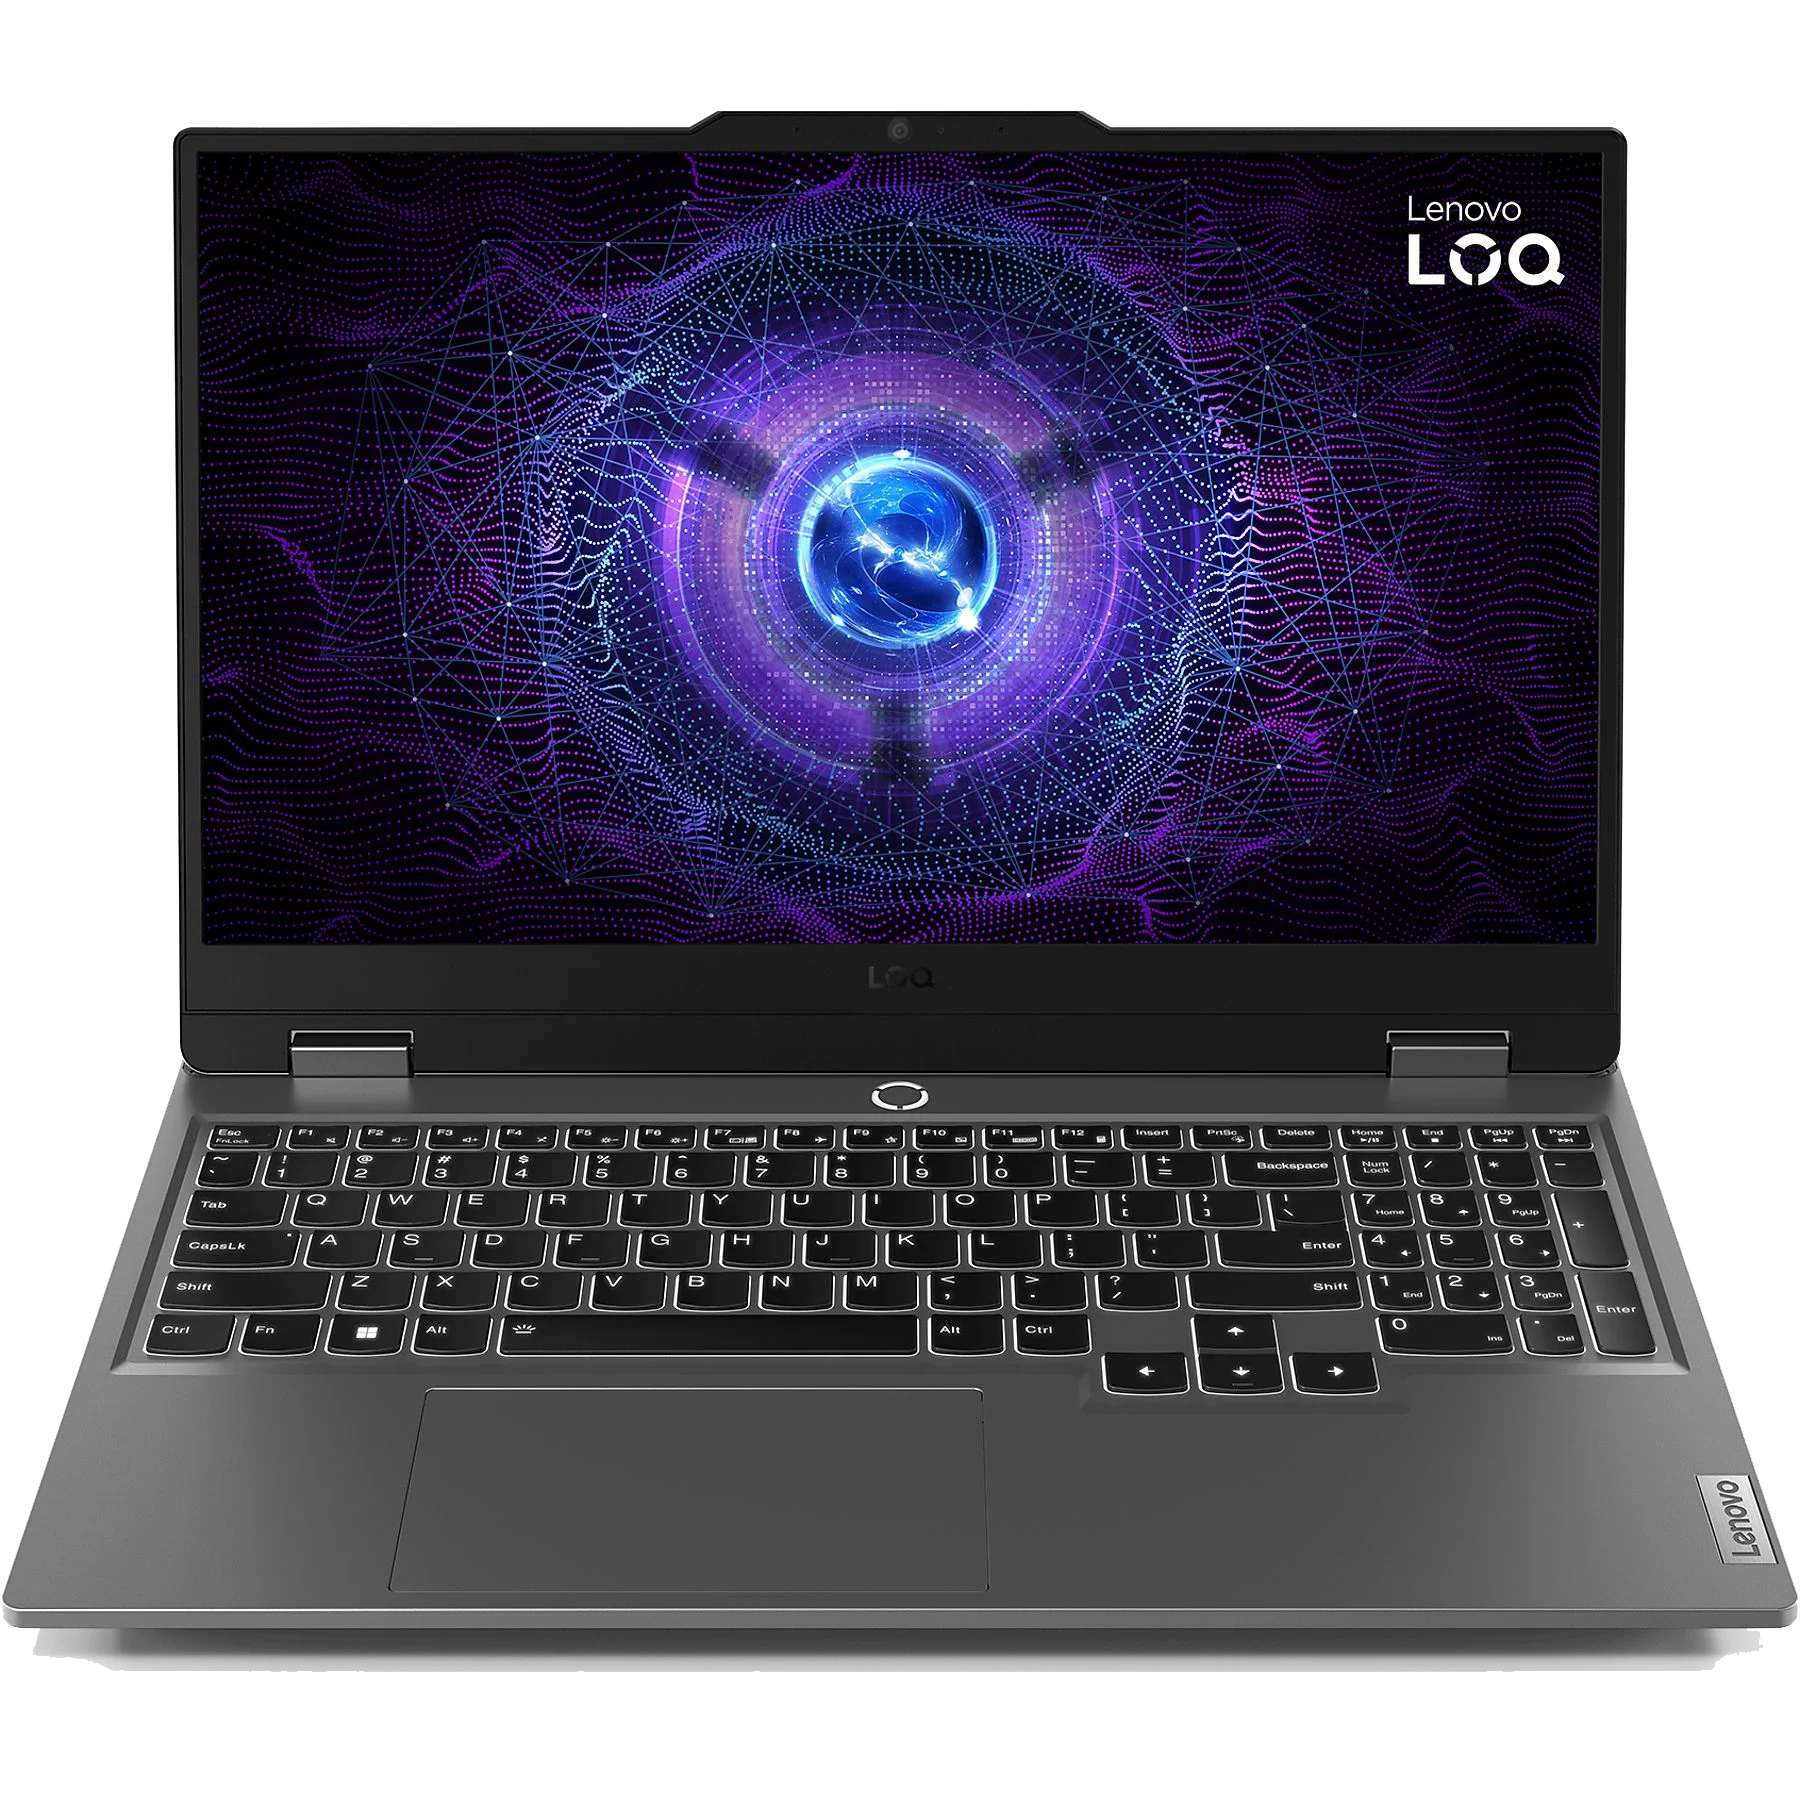
\includegraphics[width=.7\textwidth]{Images/hadwareBOM/LenovoLaptop.png}
	\caption{Lenovo Laptop}
	\textbf{Link:} \href{https://www.lenovo.com/de/de/p/laptops/loq-laptops/lenovo-loq-essential-gen-9-15-intel/83lkcto1wwde1}{Lenovo official page}
\end{figure}

\subsection*{Detailed Hardware Specifications}

\begin{table}[H]
	\centering
	\caption{Recommended Development Hardware Specifications}
	\begin{tabular}{|p{3cm}|p{5cm}|p{5cm}|}
		\hline
		\textbf{Component} & \textbf{Recommended Specification} & \textbf{Purpose in Project} \\
		\hline
		\textbf{Processor} & Intel Core i5-1235U or AMD Ryzen 5 5625U & Efficient multi-core processing for pandas operations and ARIMA model training \\
		\hline
		\textbf{Memory} & 16 GB DDR4-3200 & Comfortable handling of Walmart dataset (4,400+ time series) and multiple Streamlit sessions \\
		\hline
		\textbf{Storage} & 512 GB NVMe SSD & Fast data loading for CSV files and quick model serialization/deserialization \\
		\hline
		\textbf{Graphics} & Integrated Intel Iris Xe or AMD Radeon & Sufficient for Plotly visualizations and Streamlit interface rendering \\
		\hline
		\textbf{Display} & 15.6" Full HD (1920x1080) IPS & Clear viewing for data visualization and code development \\
		\hline
		\textbf{Connectivity} & Wi-Fi 6, Bluetooth 5.1, USB-C & Modern connectivity for development tools and cloud deployment \\
		\hline
		\textbf{Operating System} & Windows 11 Pro or Ubuntu 22.04 LTS & Stable platform with good Python ecosystem support \\
		\hline
	\end{tabular}
	\label{tab:recommended-specs}
\end{table}

\section*{Performance Analysis by Component}

\begin{table}[H]
	\centering
	\caption{Component Importance for Time Series Forecasting}
	\begin{tabular}{|p{3cm}|p{3cm}|p{7cm}|}
		\hline
		\textbf{Component} & \textbf{Importance} & \textbf{Impact on Project Performance} \\
		\hline
		\textbf{CPU} & High & Critical for ARIMA parameter optimization and Exponential Smoothing calculations. Multi-core beneficial for parallel processing \\
		\hline
		\textbf{RAM} & High & Essential for loading 4,400+ time series in memory. 16GB recommended for comfortable development \\
		\hline
		\textbf{Storage (SSD)} & Medium-High & Significantly improves data loading times and application startup. NVMe preferred over SATA \\
		\hline
		\textbf{GPU} & Very Low & Not utilized by statsmodels or pmdarima. Integrated graphics sufficient for all visualization needs \\
		\hline
		\textbf{Network} & Medium & Important for cloud deployment and accessing remote datasets \\
		\hline
		\textbf{Display} & Medium & Affects development productivity and data visualization quality \\
		\hline
	\end{tabular}
	\label{tab:performance-analysis}
\end{table}

\section*{Cloud Deployment Considerations}

\subsection*{Streamlit Cloud (Recommended)}

\begin{table}[H]
	\centering
	\caption{Streamlit Cloud Specifications}
	\begin{tabular}{|p{3cm}|p{10cm}|}
		\hline
		\textbf{Resource} & \textbf{Specification} \\
		\hline
		\textbf{CPU} & Shared CPU cores (sufficient for most use cases) \\
		\hline
		\textbf{Memory} & 1 GB RAM (adequate for single-user sessions) \\
		\hline
		\textbf{Storage} & Limited temporary storage (models loaded from repository) \\
		\hline
		\textbf{Cost} & Free tier available, paid plans for higher usage \\
		\hline
		\textbf{Advantages} & No hardware investment, automatic scaling, built-in CI/CD \\
		\hline
	\end{tabular}
	\label{tab:streamlit-cloud}
\end{table}

\subsection*{Alternative Cloud Platforms}

For organizations requiring more control or higher performance:

\begin{itemize}
	\item \textbf{AWS EC2 t3.medium}: 2 vCPU, 4 GB RAM - suitable for small teams
	\item \textbf{Google Cloud Compute e2-standard-2}: 2 vCPU, 8 GB RAM - balanced performance
	\item \textbf{Azure B2ms}: 2 vCPU, 8 GB RAM - good integration with Microsoft ecosystem
\end{itemize}

\section*{Development Environment Setup}

\subsection*{Local Development Requirements}

\begin{itemize}
	\item \textbf{Python Environment}: Python 3.12 with virtual environment support
	\item \textbf{IDE/Editor}: VS Code, PyCharm, or Jupyter Lab for development
	\item \textbf{Version Control}: Git for source code management
	\item \textbf{Package Management}: pip or conda for dependency management
\end{itemize}

\subsection*{Memory Usage Patterns}

\begin{table}[H]
	\centering
	\caption{Typical Memory Usage}
	\begin{tabular}{|p{4cm}|p{3cm}|p{6cm}|}
		\hline
		\textbf{Operation} & \textbf{RAM Usage} & \textbf{Description} \\
		\hline
		Application Startup & 200-300 MB & Base Streamlit application and library imports \\
		\hline
		Dataset Loading & 400-600 MB & Full Walmart dataset (45 stores, 4,400+ series) \\
		\hline
		Model Training & 800 MB - 1.2 GB & ARIMA parameter search and model fitting \\
		\hline
		Prediction Generation & 300-500 MB & Generating forecasts and visualizations \\
		\hline
		Peak Usage & 1.5-2 GB & Multiple concurrent operations \\
		\hline
	\end{tabular}
	\label{tab:memory-usage}
\end{table}

\section*{Budget Considerations}

\subsection*{Hardware Investment Recommendations}

\begin{table}[H]
	\centering
	\caption{Budget Options}
	\begin{tabular}{|p{3cm}|p{3cm}|p{7cm}|}
		\hline
		\textbf{Budget Range} & \textbf{Target Users} & \textbf{Recommended Approach} \\
		\hline
		€0 - €100 & Students, hobbyists & Use existing hardware + cloud deployment for intensive tasks \\
		\hline
		€400 - €700 & Small businesses, freelancers & Mid-range laptop with 16GB RAM and SSD \\
		\hline
		€700 - €1200 & Professional developers & High-performance laptop with premium build quality \\
		\hline
		€0 (Cloud-only) & Any organization & Streamlit Cloud or other cloud platforms \\
		\hline
	\end{tabular}
	\label{tab:budget-options}
\end{table}

\section*{Scalability Considerations}

\subsection*{Growing Dataset Requirements}

If planning to scale beyond the current Walmart dataset:

\begin{itemize}
	\item \textbf{10x Dataset Size}: Upgrade to 32 GB RAM, consider workstation-class CPU
	\item \textbf{Real-time Processing}: Add SSD storage in RAID configuration
	\item \textbf{Multiple Users}: Migrate to cloud infrastructure with load balancing
	\item \textbf{Enterprise Deployment}: Consider containerization with Docker/Kubernetes
\end{itemize}

\section*{Special Considerations}

\subsection*{No GPU Requirement}

Unlike machine learning projects requiring neural networks, this time series forecasting system does not benefit from GPU acceleration:

\begin{itemize}
	\item \textbf{ARIMA Models}: CPU-based calculations, no GPU libraries available
	\item \textbf{Exponential Smoothing}: Sequential algorithms not suited for parallel GPU processing
	\item \textbf{Data Processing}: Pandas operations are CPU-optimized
	\item \textbf{Visualization}: Plotly renders efficiently on integrated graphics
\end{itemize}

\subsection*{Cross-Platform Compatibility}

The recommended hardware supports all major operating systems:

\begin{itemize}
	\item \textbf{Windows 10/11}: Native Python support, good development tools
	\item \textbf{macOS}: Excellent for development, though ARM (M1/M2) may require specific package versions
	\item \textbf{Linux (Ubuntu/Debian)}: Optimal for production deployment, lightweight
\end{itemize}

\section*{Summary}

The Walmart Sales Forecasting System is designed to be hardware-efficient, requiring only modest computing resources. A mid-range laptop with 16 GB RAM and an SSD provides excellent performance for both development and local deployment. For end users, cloud deployment via Streamlit Cloud eliminates hardware requirements entirely while providing reliable access to the forecasting capabilities.

The absence of GPU requirements and the focus on efficient time series algorithms make this system accessible to a wide range of users and organizations, from students learning data science to businesses implementing forecasting solutions without significant hardware investments.